% !TEX root = ../main.tex
\chapter{Viphoger} \label{ch::viphoger}
\DndDropCapLine{A}{s a new nation, Viphoger is small. Its}
poleis are minuscule in comparison to the wilderness beyond, but their inhabitants live joyfully in their newly earned independence.

\begin{table*}[b]
\begin{DndTable}[width=\linewidth, header=Fagalian Calendar]{cXXX}
    \textbf{Month} & \textbf{Name} & \textbf{Tide} & \textbf{God} \\
    1              & Amion         & Blue          & Heliod, God of the Sun \\
    2              & Sianion       & Gold          & Ephara, God of the Polis \\
    3              & Granion       & Magenta       & Iroas, God of Victory \\
    4              & Zmivion       & Silver        & Phenax, God of Deception \\
    5              & Skenion       & Red           & Mogis, God of Slaughter \\
    6              & Danion        & Blue          & Kruphix, God of Horizons \\
    7              & Dibinion      & Gold          & Purphoros, God of the Forge \\
    8              & Ranion        & Magenta       & Athreos, God of Passage \\
    9              & Amelamion     & Silver        & Thassa, God of the Sea \\
    10             & Amelsion      & Red           & Erebos, God of the Dead \\
    11             & Amelgranion   & Blue          & Pharika, God of Affliction \\
    12             & Amelzvion     & Gold          & Nylea, God of the Hunt \\
    13             & Amelskenion   & Magenta       & Klothys, God of Destiny \\
    14             & Ameldanion    & Silver        & Karametra, God of Harvests \\
    15             & Ameldibinion  & Red           & Keranos, God of Storms \\
    16*            & Fisimmas      & White         & The Traveler, God of Luck
\end{DndTable}
\end{table*}
% * This day only occurs once every ten years.

Viphoger consists of a peninsula forming the south-western edge of the vast Whaler's Sea.
South from the sea, the land rises up to a ridge of mountains.
The lofty peaks of this ridge forms a barrier that few cross, so only rumors of the vast Dead Sea describe the land beyond.

To the west, the coastal lands become small pockets of forests crossed by a labyrinth of arid canyons, with the Zoedrem desert beyond.

The Siren's Inlet to the north is studded with islands large and small.
The largest cluster near the mainland, called the Dakra Isles, is poorly charted, and even those sailors who attempt to explore the isles return with contradictory information.
Eastward from Viphoger, the old nations of Yuadrem trade in the Whaler's Sea. % , regulated by the strong influence of the Seven Kingdoms of the Sea.

The heart of Viphoger lies in and around three poleis—cities and their surrounding territories.
Together the three poleis, Akhosh, Mephetis, and Setesh, encompass most of the population of Viphoger.
Mephetis covers the whole territory of the northeastern peninsula, Akhosh forms the frontier to the desert, and Setesh lies at the northern edge of the wild Nessian Wood.

The bands of the Uqhardu, the Vahagha, and the Pheres, roam the hills and badlands between the three poleis.
Remnants of the once great empire of Hulnar, now reduced to bandits and traders.
The mysterious leonin hunt in the valley of Oreskos, nestled between Mt. Kure and Winter's Heart.
Bughna gats and marsets dwell around the Stola Vale and the larger Nessian Wood.
And tortles live primarily in the coastal shallows of the Siren Inlet, though some manage to make comfortable homes among the gats of Mephetis.

The canyon of Katajthon, south of Akhosh, is the frontier where Akhoash soldiers clash with Treb gats.
Farther south-west is the city of Kofos, little known to Viphogerians.

The necropoleis of Asphodel and Odunos are home to the Returned --- zombie-like beings who have contracted the Illness.
Access to these lands is strictly forbidden, and is punishable by death in all three poleis.
The lands around these cities are bleak and barren, as if the Returned brought the pall of the underworld out with them into the mortal realm.

% !TEX root = ../main.tex
\subsection*{The Fagalian Calendar} \label{ssec::thefagaliancalendar}
The oth astronomers and philosophers from oldentimes established a calendar that has found massive adoption in the rest of Yuadrem.
It divides the year into fifteen months of twenty-four days, each beginning after the new Fagal.
Every ten years, an extra day is added at the end of the calendar to keep it aligned with the solar year.

The beginning of the year is considered the end of spring, so the new year begins with the summer.
Each month is associated to a tide, and is holy to a specific god.
A major festival in honor of that god is celebrated in Mephetis.
The fifth month (Skenion in Mephetis) is called Iroagonion in Akhosh, after the Iroan Games, which are held in that month every year.

% The Fagalian Calendar table summarizes the months, their lengths, and the god each is associated with.


\incgraph[documentpaper,][width=\paperwidth,height=\paperheight]{02viphoger/img/00map.png}
\newpage~\newpage

% !TEX root = ../main.tex
\subsection*{Life in the Poleis} \label{ssec::lifeinthepoleis}
Civilization in Viphoger is centered in three poleis: Akhosh, Mephetis, and Setesh.
These poleis exemplify the kins' drive to settle the land, to shape nature according to their needs, and to organize into political structures that can withstand the changing fortunes of the passing centuries.

Each polis is centered in a city but includes a wide region of surrounding territory, and each one has its own distinct society and culture.
To the people of Viphoger, ``Mephetis'' is more or less synonymous with ``Mephetians'' --- the polis isn't just the people who live in the city of Mephetis or even those who dwell in nearby villages; it is the people who follow the Mephetian way of life, wherever they might be found.

\subsubsection{Citizenship and Government}
In every polis, civic responsibility and full protection are afforded only to citizens.
Citizenship is limited to those whose parents were both citizens of the polis.
Citizens of other poleis, and their children, aren't permitted to participate in the government of the polis.
In Akhosh, citizens must meet one additional requirement: they must serve in the army.

The three poleis have different political structures, but each one has a council elected by popular vote of the citizenry.
The Twelve, Mephetis's council of philosophers, is the democratically elected ruling body of the polis.
Akhosh is ruled by a hereditary monarch who is advised by a council of elders elected by and from among the citizenry.
Similarly, Setesh's Ruling Council is formed by popular vote, and they govern the polis while its queen --- the goddess Karametra --- is absent.

\subsubsection{Trade and Currency}
Trade between Akhosh and Mephetis is constant and productive.
Caravans make the two-week journey between the poleis twice a month, aided by the Tsher river.
They carry fine Akhoshian metalwork and pottery to Mephetis, and Mephetian fabric, stonework, and fish westward.
Both poleis mint coins of copper, silver, and gold, with equivalent value.

Setesh trades with the other poleis as well, but less extensively.
Its Abora Market, just inside the city gates, is open to outsiders only on certain days, and Seteshan merchants prefer to barter goods rather than accept currency.
Despite these restrictions, Seteshan food, woodwork, and trained falcons are highly valued in the other poleis.

Aside from the other poleis, Mephetis and Setesh both trade with the dratl irds of the Vahagha band.
The irds don't work metal, so they trade woodwork, the produce of the plains, and woven blankets to the human poleis in exchange for weapons and armor.

\subsubsection{Recreation}
The people of the poleis enjoy the opportunity for some recreation, as time and money allow.

Gymnasia are popular gathering places, offering athletic training as well as space for philosophical discussion and friendly socializing.
A resident of the city might visit a gymnasium one day to exercise, the next to view a wrestling match between celebrated competitors, and the next to hear a renowned philosopher give a lecture on ethics.

Another important venue for recreation is the theater.
The works of celebrated playwrights, past and present, are regularly produced by casts of professional actors.
On occasion, a storyteller, accompanied by a small orchestra, draws crowds to a theater for a recitation of one of the great epics, such as The Sylvan Wars, The Theriad, or The Callapheia.
Such a performance might stretch over two or three days.

% !TEX root = ../main.tex
\section{Akhosh} \label{sec::akhosh}
\DndDropCapLine{}{Only victory endures.}

\hspace*{\fill} --- Akhoash motto.

The walled polis of Akhosh stands defiantly atop a precipitous cliff.
The unforgiving Katajthon canyon under it serve as a shield between its holdings and the rest of Viphoger.
Few have ever dared to attack its famed fortress, the Kolophon, and no attack has ever breached its walls.
To the residents of Viphoger, the Akhoans hold near-mythical status: feared warriors produced by a culture that centers around perfecting the mind and body for war.
Their armies have rarely tasted defeat as they expand the borders of Akhosh, seizing new lands and bounty.

\subsection*{People of Akhosh} \label{ssec::peopleofakhosh}
    For most of Akhosh's neighbors, the term "Akhoash" evokes legendary warriors, trained from birth in every martial discipline known to gatkind.
    It brings to mind songs of tight-knit martial bands, holding strong in the face of unbeatable odds.
    It sings of a great yearly competition that crowns the preeminent warrior-athlete in Akhosh, and—by extension—Viphoger.
    The majority of Akhosh's inhabitants, though, aren't members of its martial elite.
    The famed warriors of Akhosh have the means to devote their lives to studying and training in the ways of war because they rest atop a rigid social structure of serfs and servants that largely dwell beyond the Kolophon's walls.
    Those who stand at the heights of Akhoash society, or outside it, are detailed here.

    \subsubsection{The Monarchy}
        Traditionally, Akhosh is ruled by a gat monarch drawn from the lineage of lektoi.
        The monarchy passes from parent to eldest child, but any sibling or firstcousin of the heir can challenge this succession and claim the throne by besting the heir in single combat.

        Currently, the monarchy is in a state of turmoil.
        King Anax has died, and his child, Cymede, has disappeared.
        An oracle of Keranos, Cymede is said to have transformed into a pillar of fire and vanished into the wind, but until their death is certain, the lektoi are reluctant to name a new monarch.
        Anax has no other children, so the king's nephew, Taranika, acts as regent, attempting to guide the polis through what is sure to be a difficult transition.

        As if the situation weren't complicated enough, rumors have it that Anax isn't dead.
        They, or perhaps some shimmering Nyxborn simulacrum of him, has been seen at the head of squads of bughna gat hoplites, wielding an axe that billows with smoke and drips searing lava.

    \subsubsection{Lektoi}
        At the apex of Akhoash society are the lektoi, the large warrior class of Akhosh.
        Members of this class claim descent from the seven warriors who first established the Kolophon during the Sylvan wars.
        Though the families now number more than seven, each one uses an animal associated with one of the seven warriors as its symbol, either the ram, lion, horse, boar, badger, bull, or hart.
        The ram, associated with Akhosh's first king, Elektes, is commonly used as a symbol for the lektoi as a whole and for Akhoash strength, determination, and resilience.
        It is a popular theme in clothing, jewelry, and weapon ornamentation. % , and some lektoi even wear their hair braided into stylized ram horns.

        Although the lektoi claim descent from heroes, membership in this noble class isn't strictly hereditary.
        Anyone can earn a place among them by claiming a victory in the annual Iroan Games.
        More commonly, members of lektoi families lose their place of privilege if they fail to fulfill their obligation to serve in the Akhoash military.

    \subsubsection{Stratians}
        The Akhoash military is formed of wandering bands of warriors (drawn from the lektoi families) known as stratians.
        Outside the walls of the Kolophon, the stratians camp in the forests and fields, hunt game for food, and train younger warriors as they go.
        Their tasks are to search for creatures that have strayed into Akhoash territory and to protect travelers.

        Stratian forces are divided into three types of duty and armed appropriately for the task before them:

        \subparagraph{Alamon} Rugged forces of wanderers patrol Akhosh's borders, defending against invasion or attack by creatures that dwell in the mountains, foothills, and badlands around Akhoash territory.
        They are armed and armored for speed and agility, allowing them to move stealthily and strike unexpectedly.

        \subparagraph{Lukos} The most elite forces among the stratians, the so-called wolves contend with threats that the Alamon can't handle alone.
        After the guerrilla tactics of the Alamon have softened up a target, the heavily armored Lukos march to finish the task.

        \subparagraph{Oromai} The watchers are the guardians of the Kolophon who protect the fortress from invaders and maintain order within its walls.

    \subsubsection{Flamespeakers}
        Prominent spellcasters, the flamespeakers are reclusive priests of Purphoros who revere nature spirits and who inhabit fiery rifts in the mountains.

        \pagebreak

        % NOTE: At some point I should figure out how to use wrapfigure and tikzpicture together.
        \begin{tikzpicture}[remember picture,overlay]
            \node[anchor=north, yshift=0.10cm] at (current page.north) {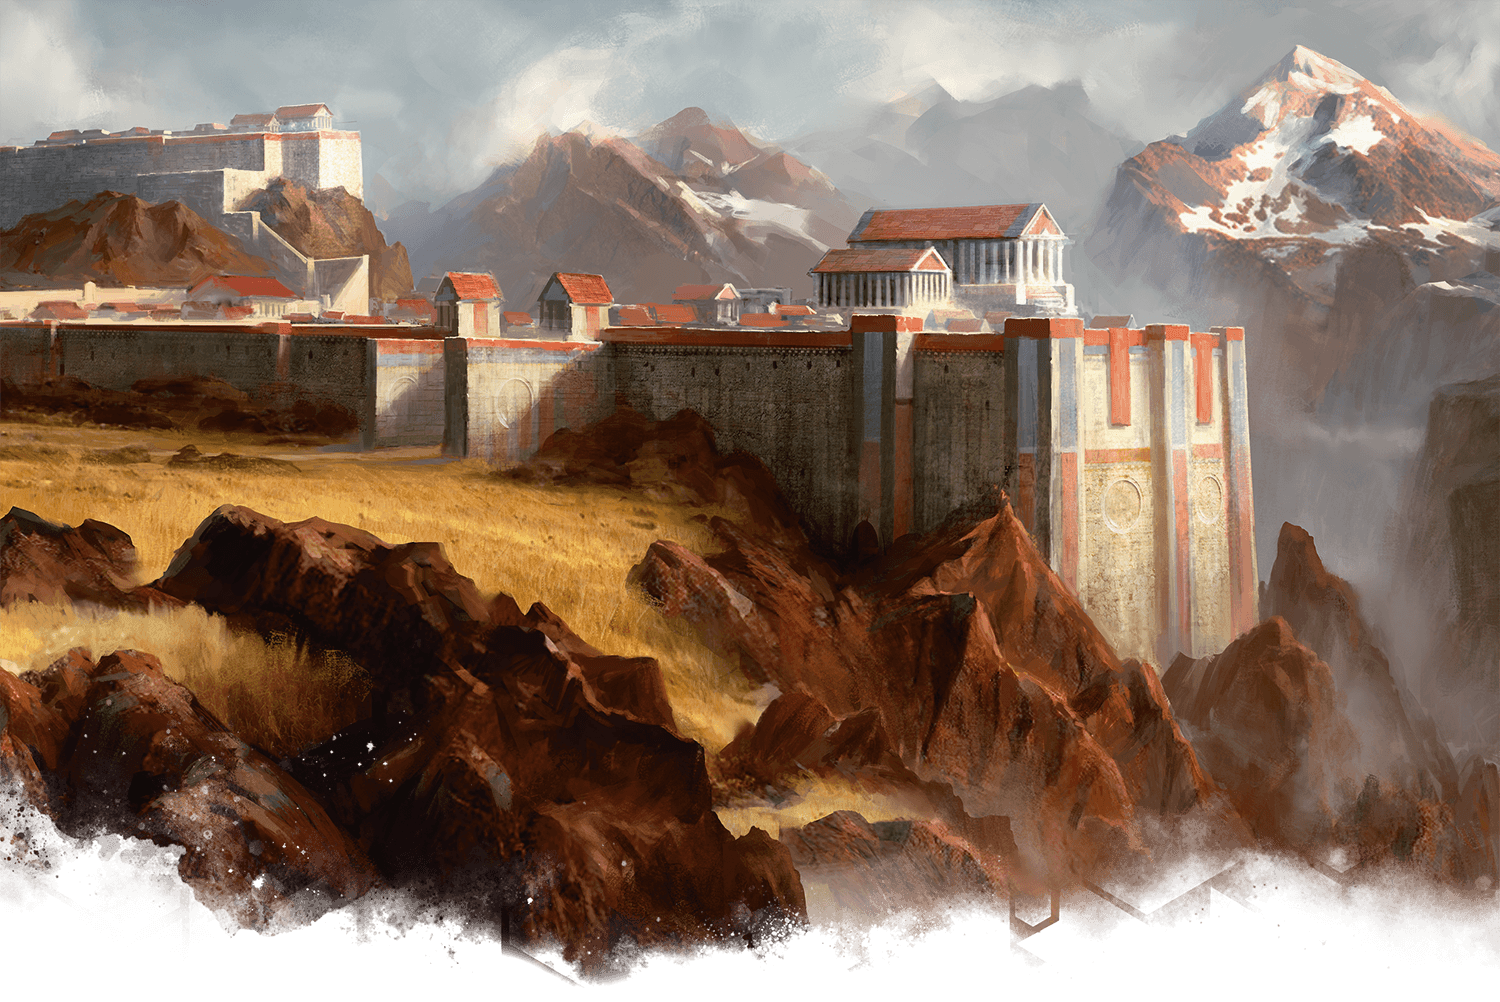
\includegraphics[width=\pdfpagewidth]{02viphoger/img/10kolophon.png}};
        \end{tikzpicture}

        \vspace{12.5cm}

        The ancient practice is viewed as primitive but powerful, and Akhoans of any background might risk making a pilgrimage into the mountains to hear a flamespeaker's prophecies.

    \subsubsection{Servants and Serfs}
        Lektoi who complete their military service with honor often retire to the Kolophon or their family estates and go about the leisured life of aristocrats.
        Their households are run by a class of servants made up of lektoi who were unable or unwilling to undertake a military career.
        These servants lack citizenship's full privileges but retain a position of some honor thanks to their class.

        Below these servants, at the bottom of Akhosh's social hierarchy, are the serfs.
        Comprising the vast majority of Akhosh's population, the serfs largely reside outside the protection of the Kolophon, laboring to grow the staple crops that support Akhosh's citizens and its trade.
        A relatively small number of serfs are skilled artisans who manage to build a more prosperous life for themselves with their crafts.
        But even these wealthier serfs can't own the land they live on, and they enjoy few rights or legal protections.

        \pagebreak~
        \vspace{12cm}

    \subsubsection{Nongats in Akhosh}
        Akhosh maintains a standoffish—and often hostile—stance toward its neighbors, particularly the treb gats of Phoberos, the leonin of Oreskos, and the dratl irds of the Pheres band.
        Members of those peoples rarely find a warm welcome in Akhoash territory.
        However, Akhoans respect prowess, loyalty, and self-sacrifice, and might welcome any who embody such virtues.
        Some stratians also seek to learn the martial practices of other peoples, and might invite individuals or small communities to Akhosh to learn their ways.

        During the Iroan Games, everyone is welcome in the stadium.
        Thousands flock to the city to witness the competition, and some take up permanent residence, celebrating the outcome of one year's games until it's time to start watching the next.

\subsection*{Features of Akhosh}
    At the center of the polis of Akhosh rises the Kolophon, a mighty fortress and the seat of Akhoash power.
    This many-tiered structure perches upon a vast cliff, which drops into a deep canyon carved by the Tsher River.
    Nature and Akhoash ingenuity conspire to make the Kolophon one of the most intimidating fortresses in Viphoger.

    Beyond the polis stretch craggy hills and canyon walls broken by narrow stretches of arable plains.
    It is a nearly impassable landscape, save for a few roads hewn through passes.
    Residents claim that only a fool would attempt to invade the heartlands of Akhosh, yet Akhoashs obsessively guard against invasion nonetheless.

    Beyond its thick walls, the streets of Akhosh are dotted with towering statues of heroes.
    Red-tiled roofs soar over square-topped sandstone columns, and holy sites dedicated to Iroas, Purphoros, and Keranos, among the other gods, are many.
    The architecture is formidable, spare, and militaristic, thick with sharp, angular shapes.

    \subsubsection{Temple of Triumph at Akhosh}
        At the heart of the walled city is the huge stadium that hosts Viphoger's greatest sporting event, the Iroan Games.
        A grand temple of Iroas stands beside it, serving as the venue for award ceremonies.
        A wide plaza connects the stadium to the city's outer gates, offering plenty of room for celebration around the annual games.

        When the stadium isn't hosting the actual Iroan Games, it is still used daily for training and for lesser athletic events.
        Many of the buildings surrounding the stadium are dedicated to serving it: smaller training facilities, providers of athletic gear, stables, and other shops.

    \subsubsection{Citadel}
        The uppermost tier of the city, perched on a rocky outcropping at the northwestern corner of the Kolophon, is the great citadel.
        The Oromai (the ``watchers'' who maintain order and defend the Kolophon) are quartered within the citadel's imposing walls, and the monarch's palace is built atop it.
        Temples of Iroas, Heliod, and Keranos also adorn the top of the citadel, the latter commissioned by the late prince Cymede, built with an open roof to give them a clear view of stormy skies.

\subsection*{Akhosh's Surroundings}
    Arable land is scattered across small plateaus and valleys in Akhosh, meaning that the serf communities that farm the land are small and just as scattered.
    Volcanic rifts, landslides, and venomous animals make travel dangerous for anyone who doesn't know the terrain, and visitors wishing to avoid suspicion from patrolling stratians would be wise to stick to the roads.

    \begin{figure}[!t] % NOTE: Maybe do something to this image so it doesn't look so underwhelming.
        \centering
        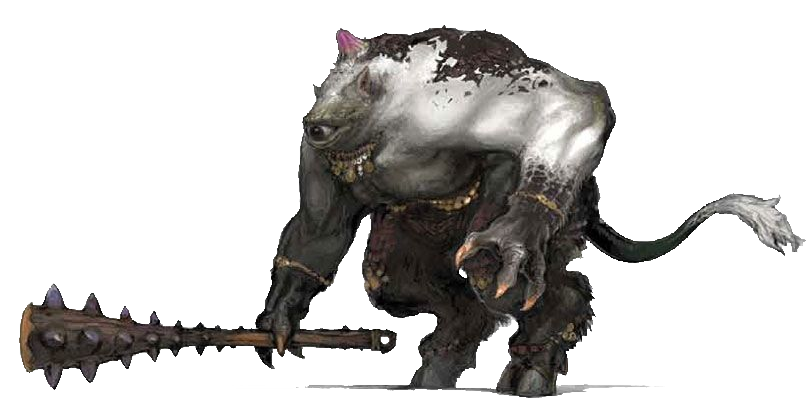
\includegraphics[width=0.48\textwidth]{02viphoger/img/10cyclops}
    \end{figure}

    \subsubsection{Outposts}
        The Alamon soldiers spend most of their time patrolling Akhosh's outlying areas, centering their patrols around scattered outposts.
        These serve as staging grounds for Alamon and Lukos units to prepare as they venture out to raid or guard against monsters and invaders.

        \subparagraph{One-Eyed Pass} The outpost in One-Eyed Pass serves to keep an Akhoash eye on the large cyclops population of the area, but the stratians also use the cyclopes to their advantage.
        Any time dangerous creatures come down from the mountains and pose a potential threat to Akhoash holdings, the Alamon harry the enemy and try to funnel them into the pass.
        The cyclopes of the pass viciously defend their territory against all intruders, weakening or even eliminating the danger before it can reach the Akhoash outpost, where the Lukos finish off any stragglers.

        \subparagraph{Pharagax Bridge} On the eastern border of Akhosh gapes a massive chasm rumored to descend all the way to the underworld and belch forth foul creatures.
        The great stone bridge that spans it is the only way into Akhosh from this direction.
        Stratians consider it a high honor to be assigned to guard the bridge.

        \subparagraph{Titan's Stairs} These stone ``stairs'', seemingly carved into the granite cliffs that protect Akhosh and haunted at all times by eerie, whistling winds, provide natural access to Akhosh.
        The stratians guard it fiercely and use it as a staging ground for invading the lowlands.

        \subparagraph{Katajthon Outposts} Several semipermanent encampments dot the rocky land between Akhosh and the rest of the Katajthon canyon.
        Fresh cadres of troops come here every month to relieve soldiers who are worn out by relentless assaults from raiders, fire-breathing dragons, and other threats.

        \subparagraph{Canyon Shrines} The Akhoashs believe that the gods are best worshiped at the places closest to Nyx --- canyon peaks.
        Small temples and shrines are found throughout Akhoash territory.
        Some are tucked in caves or nestled in crevices or canyons, while others are bare altars exposed to the elements.

    \begin{DndComment}{Myths of the Akhoash War}
        Barely a year after the end of the Sylvan War, the Hulnar empire summoned the whole host of loyal spears from the house of Tadnas to wage war on the fortified canyon polis.

        What followed was a siege that stretched on for decades.
        Whole parts of Akhosh were destroyed and rebuilt in the fighting.
        There were heroes who knew only a life of conflict, performing feats of incredible prowess for the honor of Olantin, or who awed the gods with their sleepless commitment to defending the gates of Akhosh.

        Most people today know of the event from an embellished account laid down in an epic poem, The Akhoash War.
        Authored by the great poet Vefan, the poem is considered to be a definitive accounting of the greatest war in history.
        Countless soldiers aspire to fight with the honor and purpose that inspired the heroes of the Akhoash War.
    \end{DndComment}

\subsection*{Pheres Lands}
    Between the cliffs of Akhosh and the vast grasslands of Oreskos to the south, Pheres-band dratl irds roam across the dry, hilly landscape.
    Gathered in small bands of fierce raiders, the Pheres irds plunder whatever prey they can find: merchants and other travelers moving between Akhosh and Setesh, settlers trying to eke out an existence in the region, leonin tribes, Vahagha-band irds who range too far to the south, and any others they encounter.

% !TEX root = ../main.tex
\section{Mephetis} \label{sec::mephetis} % TODO: This section needs two more pictures. Get to it!
\DndDropCapLine{}{Evil flourishes where ignorance thrives.}

\hspace*{\fill} --- Perisophia the philosopher.

\thispagestyle{empty} % Remove footer so that it doesn't clash with the image.
\begin{tikzpicture}[remember picture,overlay]
    \node[anchor=south, yshift=-0.10cm] at (current page.south) {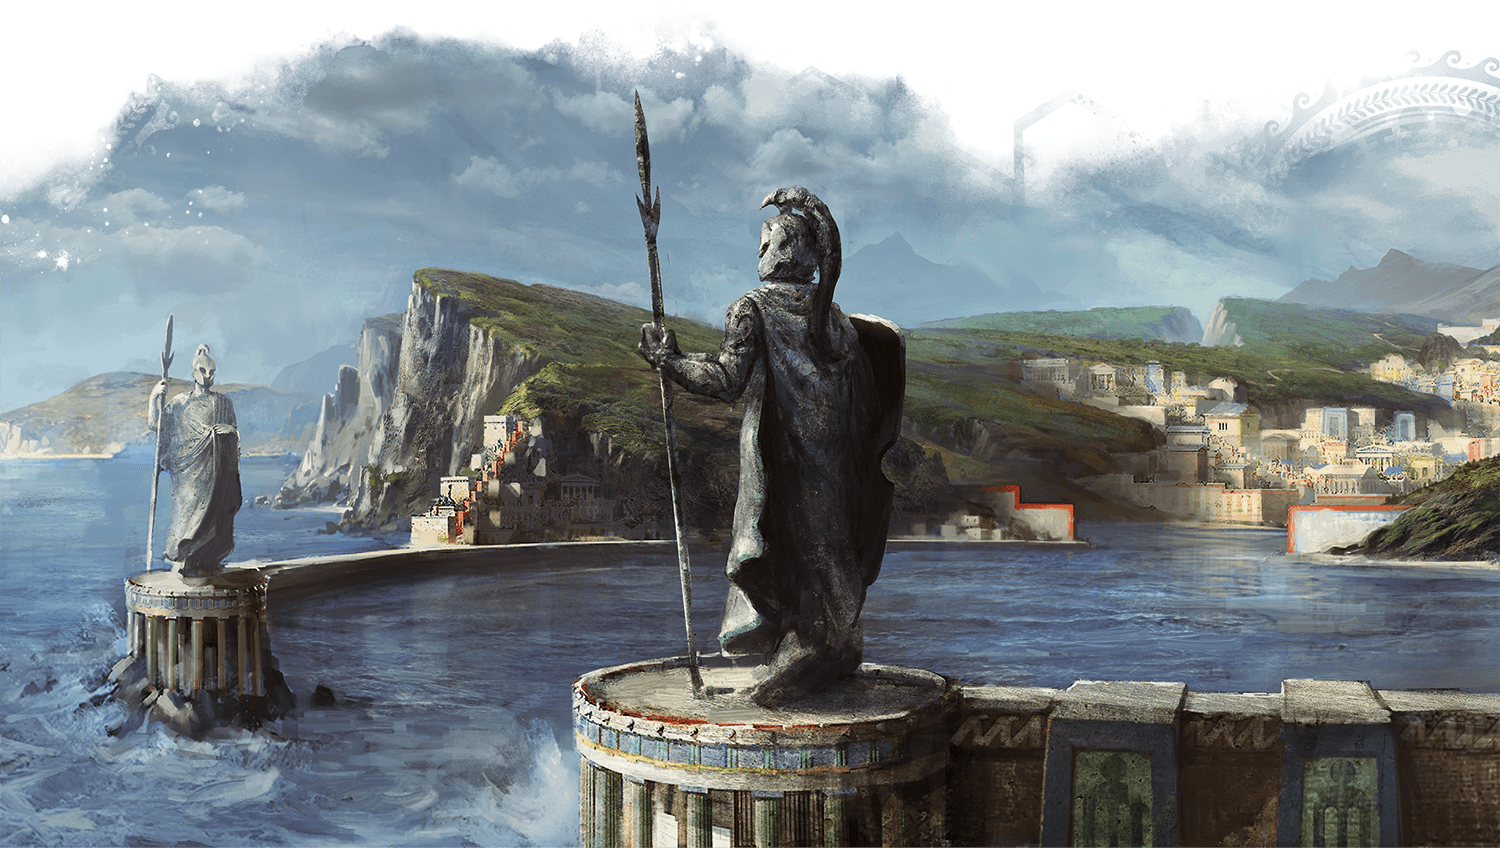
\includegraphics[width=\pdfpagewidth]{02viphoger/img/20seawall.png}};
\end{tikzpicture}

Mephetis is a polis devoted to learning, thaumaturgy, and progress.
It is the most populous city-state and home to progressive thinkers, pious thaumaturges, and wise oracles.
Born from the defeat of tyranny, to this day it pursues the ideals of free thought, societal betterment, and reinvention over stagnation and totalitarianism.

The et Agnomakhos ruled the area that is now Mephetis for centuries.
Impressing those they conquered into their legions, Agnomakhos aggressively expanded their kingdom, spreading it as far as the mountains to the south and the desert to the west.
Ultimately, though, the heroes Kynaios and Tiro overthrew the et.
From the kingdom's ruins rose Mephetis, a land that endeavors to reject cruelty and oppression throughout the world, and guards against hypocrisy within its own borders.

For a time, Kynaios and Tiro ruled Mephetis, striving to govern in accordance with the highest philosophical and ethical principles, which ultimately led them to relinquish their power and establish a philosopher-led republic.
After the kings' deaths, the council of scholars known as the Twelve took up rule of the polis, with the sage Elpidios serving as the senior member.

\newpage

\subsection*{People of Mephetis}
    The people of Mephetis take pride in their city's grand architecture, especially the great temples to the gods.
    They value philosophy and other intellectual pursuits, especially the practice of thaumaturgy.
    Mephetis's army is known for its discipline and its piety, and its navy is unparalleled.
    The city observes every one of the gods' holy days in various ways, and most residents try to live as the gods demand.

    Rich fields and the bounty of the sea support most people throughout Mephetis.
    The people have reputations for being accomplished weavers, skilled sailors, and cunning merchants.
    Books and literacy are also common throughout the land, and the work of scribes, cartographers, musicians, and storytellers is well regarded.
    The people of Mephetis believe themselves to be the inheritors of a heroic tradition, and each person owes it to themselves and to society to strive for greatness.
    Beyond Mephetis's common folk, a few groups that hold noteworthy standing are detailed here.

    \subsubsection{The Twelve}
        A council of philosophers called the Twelve serves as the ruling body of Mephetis.
        They are elected by popular vote among the citizens of Mephetis and serve for terms of four years at a time.
        They are supposed to govern by philosophical principles of justice and social order, and many of them do strive to uphold the highest ideals in their decisions.
        Others are more grimly realistic, and a few are deeply corrupt, serving only their own interests.

        \newpage

        The most senior member of the council is recognized as its leader, responsible for bringing the assembly to order and moderating its debate.
        Currently, this position is held by the renowned philosopher and orator named Perisophia.

    \subsubsection{Philosophers}
        Though they aren't necessarily heroic, philosophers are highly valued in Mephetis, which is renowned as the center of philosophical thought.
        They form a privileged class, often coming from wealthy families but also supported by stipends from the polis's academies and their own students.
        Different philosophical schools hold political as well as intellectual power in the polis, with five schools of philosophy dominating Mephetian discourse.

        \subparagraph{Elpidinas} Following the gold tide, Perisophia's optimistic Elpidian school currently predominates Mephetian thought and politics, carrying on the works of the heroic Epharan oracle Elpidios.
        The Elpidian school strives to put thaumaturgy and philosophy to use in improving the lives of all  Mephetians.
        Elpidian mages embrace magic in all its forms.

        \subparagraph{Formalists} Heralds of the indigo tide, formalist philosophers believe in a realm populated by abstract entities such as numbers and theories.
        They focus their efforts on trying to improve the moral fabric of the polis, hoping to create the ideal society, where people live together in peace, and where war and crime disappear.

        \subparagraph{Uremideans} Scholars of the blue tide, this school emphasizes logical reasoning, rhetorical excellence, and theories of ethics and virtue.
        Uremideans are eminently practical governors who seek to balance ethical ideals and realistic necessities.

        \subparagraph{Nykleans} Acolytes of no tide, nyklean philosophers teach that reason or destiny underlies all of reality, so that everything that takes place must unfold just as it does.
        These philosophers train themselves to accept and endure whatever befalls them, enjoying good fortune but not grieving its loss.

        \subparagraph{Anapsians} Followers of the red tide, anapsian philosophy embraces the fine delights of life: the pleasures of love and friendship, fine food and drink, art and music.
        Anapsians have few strong opinions about governance, except that an ultimate good end should be kept front of mind in all decision.

    \subsubsection{Thaumaturges}
        Mephetians view thaumaturgy as one of the greatest art forms, and they call the most accomplished mages thaumaturges or ``wonder workers''.
        Many Mephetian mages are trained at the elite academy of the Dekatia, but countless smaller schools and private tutors teach the magical arts.
        These lessons in thaumaturgy typically include a well-rounded education in the sciences and philosophy.
        Some thaumaturges find their magical studies aligning with popular Mephetian philosophies and choose the schools of magic they focus on based on such teachings.

        The mark of a true thaumaturge, though, is a gift or positive omen from the gods; even the most accomplished student of thaumaturgy can't earn the title without such a sign of divine approval.
        One mage might receive the gift of a spear from Heliod, another could receive a clockwork owl from Ephara, and still another might experience a wild, creative vision from Keranos.

    \subsubsection{The Reverent Army}
        The hoplites of Mephetis practice battlefield tactics in an environment saturated with religious devotion.
        The military force of the polis is called the Reverent Army, and aims as much to exalt the glory of the pantheon as to defend Mephetis.
        The soldiers are clever and resourceful, believing their piety leads the gods to smile upon them.
        More likely, though, their extensive training in battlefield tactics and thaumaturgy gives them an edge over other soldiers, with most Mephetian hoplites knowing at least a little magic.

    \subsubsection{Nongats in Mephetis}
        Mephetis strives to be a beacon to all of Viphoger's people.
        Well-intentioned members of any culture are welcome on Mephetis's streets, and the polis's people work to earn the trust of their neighbors.

        Of all the poleis, Mephetis has the closest relationship with the tortles of the Siren Inlet.
        Several communities of tortles consider the harbors of Mephetis and secluded coastal sanctuaries their home.
        Many take part in work near and under the water that other peoples are ill-suited to, but increasingly tortles find work not related to the sea, with tortle restaurants, chemists, and members of the Reverent Army being increasingly common.

        Mephetis maintains a fragile peace with the irds of the Vahagha band, engaging in regular trade.
        It's not uncommon for small groups of dral irds to set up shop in the polis market for short periods, though few spend more than a night or two in the city, most finding it claustrophobic at best.

        Few leonin journey to Mephetis, knowing little of the land beyond what their stories remember of Agnomakhos's tyranny.
        Even an age after the et's rule, most leonin view Mephetis as a cursed place.
        Those few who have traveled to the polis in recent years find it changed, with great potential for trade and cooperation, but no Mephetian or leonin has yet initiated an official dialogue between the two peoples.

        Most bughna gats have little patience for Mephetian philosophy, visiting largely out of curiosity or on elaborate larks.
        treb gats are rarely seen in Mephetis, though those who visit with peaceful intentions are welcome.

\subsection*{Features of Mephetis}
    The architectural and academic marvels of Mephetis testify to the achievements of civilized gats.
    The streets are paved with bricks made in interlocking geometric shapes, meant to demonstrate principles of both mathematics and thaumaturgy.
    Grand temples line the streets, testifying to the Mephetians' devotion to the gods.
    These rise as both mighty bastions dedicated to individual deities and various neighborhood shrines devoted to the pantheon as a whole.

    Inside the city, the wild lands feel like a remote threat.
    Perils from the sea present more obvious dangers, but a great sea wall protects the polis's port on the bay, while a lengthy channel cuts through the surrounding land to reach Mephetis Bay from the Whaler's Sea.

    \subsubsection{Pyrgnos}
        Many Mephetians speak of the ``edifice of knowledge'', referring in the abstract to the sum of all learning and scholarship.
        Every citizen is expected to help improving this edifice for the good of the polis, whether through philosophical exploration, advancements in magical technique, investigation into the nature of the gods, or perfection of techniques in crafting and trade.

        But the edifice of knowledge in Mephetis is a literal structure as well as a metaphorical one: the Pyrgnos is a glowing stone tower standing near the coast.
        It is literally formed from the collected learnings of the polis, recorded on carved stone tablets.
        At night, the top of the Pyrgnos shines like a lighthouse where the sea wall meets the shore, gleaming on the waters of the Siren Sea.

        A decade ago, the Pyrgnos was partly demolished by a kraken that attacked the city, but it has been repaired and continues to grow, reflecting the continued learning of the polis's citizens.

    \subsubsection{The Dekatia}
        Mephetis boasts many centers of learning, but the preeminent academy for philosophers and mages is the Dekatia.
        Students who display remarkable promise over the course of their earlier education can go on to spend up to ten years in arduous training at the Dekatia, apprenticed to master priests, thaumaturges, philosophers, and military heroes.
        Those who manage to complete this decade of training are renowned as the wisest of the wise and the bravest of the brave, combining all the essential learning of the polis into one package.

    \subsubsection{The Observatory}
        The Observatory is a tall viewing platform and a windowed structure offering a splendid view of the sky, renowned as a place to study the cosmos.
        Special crystals shaped by thaumaturges and blessed by the oracles of the gods enhance the view, making it easier for observers to see the workings of the gods among the stars and constellations.
        Priests, mages, and philosophers interpret what they see in the Observatory as signs and omens from the gods.

\subsection*{Mephetis's Surroundings}
    Mephetis sits on the coast of the Whaler's Sea, surrounded by rivers, sparse woodlands, and vast, stepped grasslands.
    Fields of barley provide sustenance to Mephetians and their animals.
    Well-trod roads wind their way through the region, but most locals travel along the coast in simple boats.

    \subsubsection{Mephetian Holdings}
        The polis of Mephetis embodies the heart and mind of what it means to be Mephetian, but the polis's lands also includes numerous other settlements and wildernesses.
        The people who live in these holdings are no less Mephetians than the inhabitants of the city, and they share the values of other Mephetians even if their lifestyle affords them little opportunity to study magic and philosophy.

        \subparagraph{Avtrisos} This small walled city is famous for Ephara's intervention to protect it from an illhevi, their face coming to life on the marble wall and making the barrier grow so tall that the illhevi couldn't get through.
        Avtrisos now has Ephara's face on nearly every building and wall in the entire city in gratitude.

        \subparagraph{Bjokesh} Bjokesh is a small coastal town that would be completely unremarkable, except that it's accumulated a truly impressive library.
        The bulk of the town's economy revolves around maintaining the library and meeting the needs of travelers who come to visit it.

        \subparagraph{Krinnos} Renowned as the home of Anapse, the ird philosopher who founded the Anapsian school, the village of Krinnos attracts many philosophers who share Anapse's delight in the pleasures of a simple life.

        \subparagraph{Listes} Listes is a fortress marking the southwestern border of the polis.
        The civilian population is hardly less disciplined than the members of the Reverent Army stationed there, and the whole population observes Iroas's holy days together.

        \subparagraph{Natumas} The residents of Natumas are famous for training sea animals as skillfully as Seteshans train land and air animals.
        They train sea snakes, dolphins, and even sharks on a few occasions to be combatants, working animals, aquatic mounts, and companions.

        \subparagraph{Neshantin} Though they are regarded as Mephetians, the people of Neshantin view themselves as citizens of Olantin --- a coastal polis that long ago vanished into the sea.
        According to legend, an angry Heliod smote the polis with their spear, sinking it in punishment for its people's utter hubris.
        The fact that the Neolantians were spared this fate, they say, is evidence of their humility, and they take special care in their sacrifices to Heliod.

        \subparagraph{Oxus} Oxus is a quiet town with a notably wealthy population, consisting largely of merchants who have retired from trade with large fortunes at their disposal.
        The tomb of Kynaios and Tiro also stands in the center of the town, the subject of many local legends.

        \subparagraph{Phratsh} A small fishing village, Phratsh is most noted as being the literal "end of the road" for travelers venturing south from Mephetis.
        The rugged lands beyond are rocky and scattered with forgotten ruins.

        \subparagraph{Sitrum} This coastal town is known for the way many of its buildings are on stilts to accommodate the changing tides.
        Sitrum is famed for its skilled shipwrights.

        \subparagraph{Thestre} The village of Thestre is little more than a crossroads, but it's notable for its temple to Karametra.
        The site draws farmers from the region who offer a portion of their crops to the god of agriculture.

\newpage~\pagebreak % TODO: Add more stuff here.


% TODO: ADD THESE AT SOME POINT.
% \subsection*{Pheres Lands}
%     Between the cliffs of Akhosh and the vast grasslands of Oreskos to the south, Pheres-band dratl irds roam across the dry, hilly landscape.
%     Gathered in small bands of fierce raiders, the Pheres irds plunder whatever prey they can find: merchants and other travelers moving between Akhosh and Setesh, settlers trying to eke out an existence in the region, leonin tribes, Vahagha-band irds who range too far to the south, and any others they encounter.

% \subsection*{Myth of the Akhoash War}
%     Barely a year after the end of the Sylvan War, the Hulnar empire summoned the whole host of loyal spears from the house of Tadnas to wage war on the fortified canyon polis.
%
%     What followed was a siege that stretched on for decades.
%     Whole parts of Akhosh were destroyed and rebuilt in the fighting.
%     There were heroes who knew only a life of conflict, performing feats of incredible prowess for the honor of Olantin, or who awed the gods with their sleepless commitment to defending the gates of Akhosh.
%
%     Most people today know of the event from an embellished account laid down in an epic poem, The Akhoash War.
%     Authored by the great poet Vefan, the poem is considered to be a definitive accounting of the greatest war in history.
%     Countless soldiers aspire to fight with the honor and purpose that inspired the heroes of the Akhoash War.
